% Clean CV/Resume Template, by Bennet B <dev@bennet.cc>
% CC0, Public-Domain
% 
% Permission is hereby granted, free of charge, to any person obtaining a copy
% of this template and associated files (the "Template"), to deal
% in the Template without restriction, including without limitation the rights
% to use, copy, modify, merge, publish, distribute, sublicense, and/or sell
% copies of the Template, and to permit persons to whom the Template is
% furnished to do so, subject to the following conditions:
%
% The above copyright notice and this permission notice shall be included in all
% copies or substantial portions of the Template.
%
% THE TEMPLATE IS PROVIDED "AS IS", WITHOUT WARRANTY OF ANY KIND, EXPRESS OR
% IMPLIED, INCLUDING BUT NOT LIMITED TO THE WARRANTIES OF MERCHANTABILITY,
% FITNESS FOR A PARTICULAR PURPOSE AND NONINFRINGEMENT. IN NO EVENT SHALL THE
% AUTHORS OR COPYRIGHT HOLDERS BE LIABLE FOR ANY CLAIM, DAMAGES OR OTHER
% LIABILITY, WHETHER IN AN ACTION OF CONTRACT, TORT OR OTHERWISE, ARISING FROM,
% OUT OF OR IN CONNECTION WITH THE TEMPLATE OR THE USE OR OTHER DEALINGS IN THE
% TEMPLATE.
%
% based on Modern CV by Habib Semouma
% https://www.overleaf.com/latex/templates/modern-cv-slash-resume-template/vjrqdkpjckwj
%
% 
\documentclass[oneside]{article}

\usepackage{fontspec}
\usepackage{wallpaper}
\usepackage{geometry}
\usepackage[
    unicode=true,
    bookmarks=true,
    bookmarksnumbered=false,
    bookmarksopen=true,
    bookmarksopenlevel=1,
    breaklinks=false,
    pdfborder={0 0 0},
    backref=false,
    colorlinks=false
    ]{hyperref}
\usepackage{lastpage}
\usepackage{hyphenat}
\usepackage{hyphsubst}
\usepackage{tabularx}
\usepackage{moresize}
\usepackage[document]{ragged2e}
% \usepackage{parskip}

\usepackage[scaled]{helvet}
\usepackage{fontawesome5}
\usepackage{academicons}
\usepackage[defaultfam,tabular,oldstyle]{montserrat}
\usepackage[T1]{fontenc}
\renewcommand*\oldstylenums[1]{{\fontfamily{Montserrat-TOsF}\selectfont #1}}

\usepackage{titlesec}
\usepackage{xcolor}
\usepackage{tikz}

\setlength{\parindent}{0pt}
\titleformat{\section}{\normalfont}{}{0pt}{}

\renewcommand{\arraystretch}{1.4}

\setlength\fboxrule{0pt}
\setlength\fboxsep{12pt}
% \setlength{\parskip}{.5\baselineskip plus 2pt}
% \renewcommand{\baselinestretch}{1.1}

\titlespacing{\section}{0pt}{1.5ex plus .1ex minus .2ex}{1pc}

%\tolerance=1
%\emergencystretch=\maxdimen
\hyphenpenalty=10000
\hbadness=10000

\newcolumntype{Y}{>{\RaggedRight\arraybackslash}X}

% Change PDF Meta Info here
\hypersetup{
    pdftitle={Mario Grandi - CV - English},
    pdfauthor={Mario Grandi},
    pdfsubject={CV}
}

% Paper size
\geometry{
    a4paper,
    left=0pt,
    right=0pt,
    top=0pt,
    bottom=0pt,
    nohead,
    % includefoot,
    nomarginpar
}

% Background Color of the Sidebar Column
\definecolor{sidebg}{cmyk}{1, 0.02, 0, 0.56}
% Background Color of the Main Column
\definecolor{mainbg}{cmyk}{0, 0, 0.07, 0.04}

% Text Color of the Main Column
\definecolor{maintext}{cmyk}{1, 0.02, 0, 0.8}
% Text Color of the Sidebar Column
\definecolor{sidetext}{cmyk}{0, 0, 0.07, 0.04}

\pagecolor{mainbg}

% Build custom made command for quick employment history inputs
\newcommand{\empitem}[7]{
        {\large \textbf{#1}} \\
        {{\fontseries{medium}\selectfont #2}}\\
        {{\fontseries{light}\selectfont #3}} \hfill
        {\scshape\fontseries{light}\selectfont\footnotesize #4 \textendash{} #5 #6} 
        #7
}

\begin{document}
%\setlength{\topskip}{0pt}\setlength{\footskip}{0pt}%
\fcolorbox{red}{sidebg}{%
    \begin{minipage}[t][\textheight-2\fboxsep-2\fboxrule][t]{\dimexpr0.4\textwidth-2\fboxrule-2\fboxsep\relax}
        \color{sidetext}
        %%%%%%%%%%%%%%%%%%%%%%%%%%%%%%%%%%%%%%%%%%%%%%%%%%%%
        % YOUR NAME, PRONOUNS, OCCUPATION(s), AND HEADSHOT
        {\bfseries\scshape\HUGE Mario} \\
        {\bfseries\scshape\Huge Grandi}
        \vspace{.3cm} \\
        \begin{center}
            \begin{tikzpicture}
            \clip (0,0) circle (3.5cm) node[anchor=center] {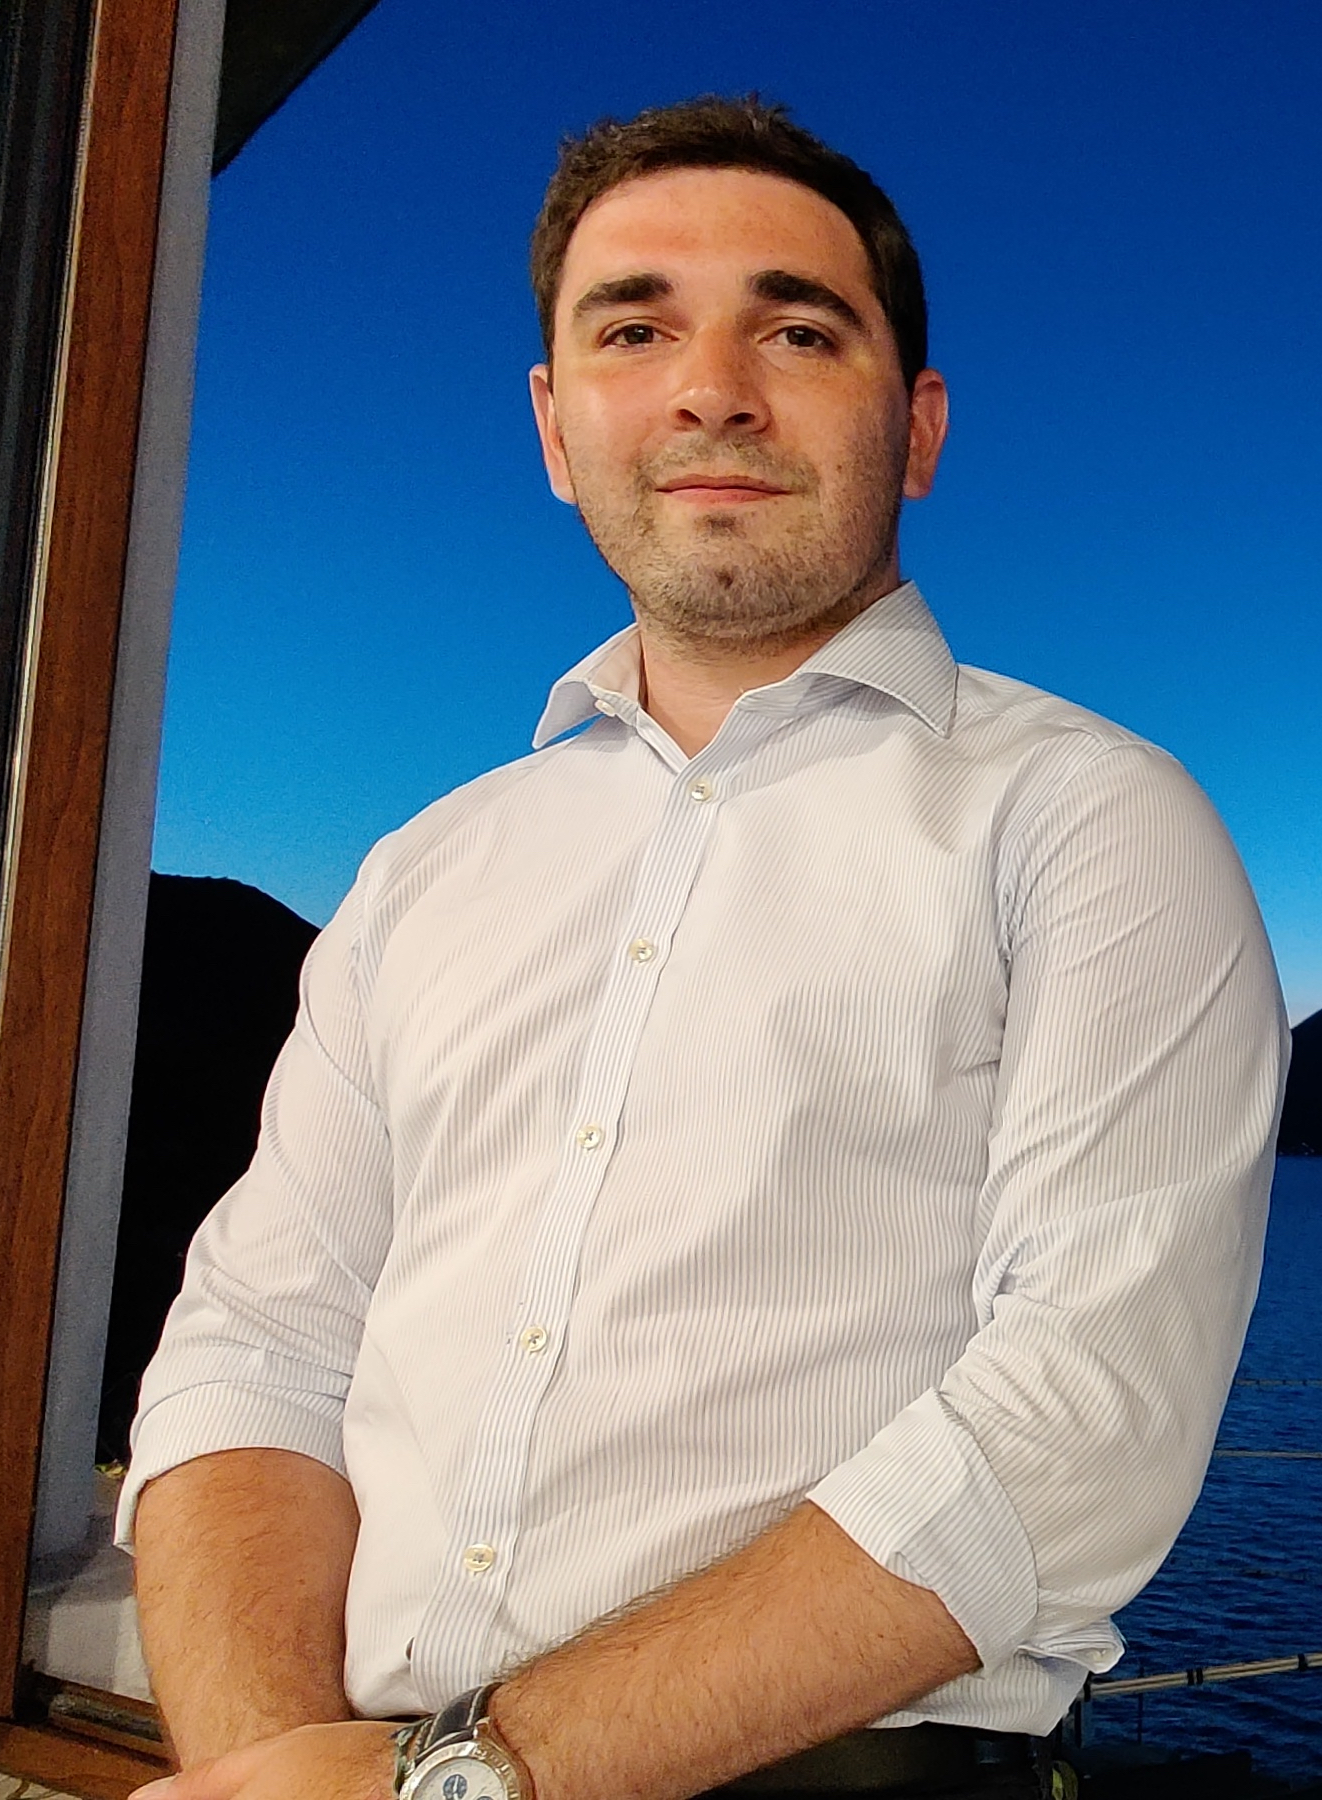
\includegraphics[trim=0cm 0cm 0cm 0cm, clip=True, width=7cm]{mario_grandi.jpeg}}; 
            \end{tikzpicture}
        \end{center}
        \vspace{.3cm}
        %%%%%%%%%%%%%%%%%%%%%%%%%%%%%%%%%%%%%%%%%%%%%%%%%%%%
        % YOUR PERSONAL INFROMATION
        \phantomsection{}
        \addcontentsline{toc}{section}{Personal info}
        \section*{\large Personal info}
        \begin{tabular}{cl}
            \faWhatsapp{}      & +65 (0)93539461 \\
            \faPhone{}      & +44 (0)7999206347 \\
            \faEnvelope{}   & \href{mailto:dr.mario.grandi@gmail.com}{dr.mario.grandi@gmail.com} \\
            \faMapMarker{}  & Singapore \\
                            %& 45a Borough Street, Brighton\\
                            %& BN1 3BG, United Kingdom \\
        \end{tabular}
        \vspace{.3cm} \\
        \rule{\linewidth}{0.4pt} \\
        %%%%%%%%%%%%%%%%%%%%%%%%%%%%%%%%%%%%%%%%%%%%%%%%%%%%%%%%%
        % YOUR LINKS, YOU MAY ALSO ADD A PERSONAL WEBSITE OR PORTFOLIO
        \phantomsection{}
        \addcontentsline{toc}{section}{Links}
        \section*{\large Links}
        \begin{tabular}{cl}
            \faGlobe{}     & \href{https://mg380.github.io}{https://mg380.github.io}\\
            \faGithub{}   & \href{https://github.com/mg380}{https://github.com/mg380} \\
            \faLinkedin{} & \href{https://www.linkedin.com/in/mario-grandi/}{www.linkedin.com/in/mario-grandi} \\
            \aiOrcid{}     & \href{https://orcid.org/0000-0002-5924-2544}{0000-0002-5924-2544} \\
        \end{tabular}
        \vspace{10pt} \\
        \rule{\linewidth}{0.4pt} \\
        %%%%%%%%%%%%%%%%%%%%%%%%%%%%%%%%%%%%%%%%%%%%%%%%%%%%%%%%%%%%
        % YOUR SKILLS
        % Add/Remove as seen fit, Icons: https://packages.oth-regensburg.de/ctan/fonts/fontawesome5/doc/fontawesome5.pdf
        \phantomsection{}
        \addcontentsline{toc}{section}{Skills}
        \section*{\large Skills}
        \begin{tabularx}{\textwidth}{cY}
            \faCode        & Python \textendash{} C++ \textendash{} Bash \textendash{} MySQL \textendash{} SQL \textendash{} AWS \textendash{} Git/GitHub/GitLab \textendash{} Microsoft Excel \\
            \faToolbox     & TensorFlow \textendash{} Keras \textendash{} Pandas \textendash{} Scipy \textendash{} Numpy \textendash{} OpenCL \textendash{} pyOpenCL \textendash{} OpenMP \textendash{} Vitis HLS \\ 
            \faCogs      & Data Science \textendash{} Machine Learning \textendash{} Bayesian Statistics \textendash{} linear/non-linear regression \textendash{} Survey Sampling \textendash{} Monte Carlo Simulations \textendash{} Distributed Computing \textendash{}  Big-Data Analysis \textendash{} Data Visualisation \textendash{} Communication \textendash{} Teamwork \\
            \faPen        & \LaTeX\hspace{0pt} \textendash{} Microsoft Studio Office \textendash{} Keynote\\
            \faLaptopCode  & Linux \textendash{} Windows \textendash{} macOS \\
        \end{tabularx}
        \vspace{1pt} 
        \\
        \rule{\linewidth}{0.4pt}\\
        %%%%%%%%%%%%%%%%%%%%%%%%%%%%%%%%%%%%%%%%%%%%%%%%%%%%%%%%%%%%%%%%
        % GRADESCALE (if nesseary, e.g. if you apply abroad, where scales 
        % are different. You should at least provide, what the best possible
        % grade and what the worst possible grade is)
    \end{minipage}
}
\hfill
\fcolorbox{red}{mainbg}{%
    \begin{minipage}[t][\dimexpr\textheight-2\fboxrule-2\fboxsep\relax][t]{\dimexpr0.6\textwidth-2\fboxrule-2\fboxsep\relax}
        \color{maintext}
        %%%%%%%%%%%%%%%%%%%%%%%%%%%%%%%%%%%%%%%%%%%%%%%%%%%%%%%%%%
        % WORK EXPERIENCE
        \phantomsection{}
        \addcontentsline{toc}{section}{Profile}
        \section*{\scshape\Large Profile \hrulefill}
        %A dedicated professional with a PhD in Experimental Particle Physics and more than 5 years of hands-on experience in data analysis, machine learning, and software development. I spearhead technical and analytical projects to deliver actionable insights and bring a proven track record of leveraging expertise in data visualization, big data technologies, and collaborative teamwork to solve a wide variety of complex challenges. I am eager to further enhance my skills and make meaningful contributions to a dynamic environment.
        
        %With a strong scientific background underpinned by a PhD in Physics and a formation as a data scientist and statistical analyst, I spearhead technical and analytical research projects to deliver actionable insights into green energy technologies. I bring a proven track record in statistical analysis, machine learning, software algorithm development, data visualisation, and collaborative teamwork to solve a variety of complex challenges. I am eager to enhance my skills further and make meaningful contributions towards a better and more sustainable environment. 
        
        I spearhead technical and quantitative research projects, leveraging my experience in Bayesian statistics and data science to deliver actionable insights. I bring a proven track record in statistical analysis, machine learning, software algorithm development, data visualisation, and collaborative teamwork to solve a wide variety of complex challenges. I am eager to enhance my skills further and make meaningful contributions to a dynamic environment.
        %%%%%%%%%%%%%%%%%%%%%%%%%%%%%%%%%%%%%%%%%%%%%%%%%%%%%%%%%%
        % WORK EXPERIENCE
        \phantomsection{}
        \addcontentsline{toc}{section}{Employment History}
        \section*{\scshape\Large Employment History \hrulefill}
%
        \empitem{Research and Analytics Lead}
        {QA-UK Ltd (Renewable Energy Technologies)}
        {London, United Kingdom}
        {May 2023}
        {ongoing}
        {}
        {
        \begin{itemize}
            \setlength{\itemsep}{-3pt}
            %\item Spearheaded the R\&D and data analysis of the full green technologies portfolio, to find out-of-the-box solutions and directly support business decision-making.
            \item Spearheaded quantitative research, planning, development, implementation, and data analysis of the full QA-UK green technologies portfolio, to find out-of-the-box solutions and directly support business decision-making.
            %\item Led a multi-disciplinary startup team in the development of green technology solutions including solar, wind, carbon capture, and green tech analytics by leveraging HPC computing infrastructures to generate valuable insights.
            \item Led a multi-disciplinary team in developing and analysing sustainable energy solutions prototypes, leveraging AWS and HPC systems to accelerate complex simulations, test models, reduce costs, and generate valuable insights.
            %\item Negotiated the implementation of software license extension, delivering 25\% additional simulation time at no extra cost.
            \item Effectively communicated and advised investors and partners, ensuring additional monetary contributions towards the continued research of our green energy technology initiatives. 
            %\item Led the testing and analysis of a prototype for a multi-million dollar green energy project and presented results to investors and stakeholders.
        \end{itemize}
        }
%
        \empitem {Statistical Production Analyst (Development lead)}
        {Office for National Statistics}
        {Titchfield, United Kingdom}
        {Sept 2022}
        {Mar 2023}
        {}
        {
        \begin{itemize}
            \setlength{\itemsep}{-3pt}
            \item Oversaw the development of the UK trade finance of services analysis and production team, leading the enhancements to the quantitative model software used to inform the national GDP and drive government decision-making.
            \item Supervised refinement of pre- and post-analysis scripts, resulting in over 50\% increase in productivity and setting a new standard for internal coding practices.
            \item Detailed requirements and user stories on JIRA using AGILE methodology, orchestrating the analysis system upgrade and migration to a Python-based Hadoop environment.
            \item Strengthened quantitative statistical analytical capabilities and operational efficacy of the system by identifying areas of improvement in the analysis structure, thus improving data quality.
            \item Utilised Tableau and other visualisation methods to effectively communicate findings to key stakeholders and successfully drive project outcomes
        \end{itemize}
        }
%
        \empitem{Post-Doctoral Research Fellow}
        {University of Sussex}
        {Brighton, United Kingdom}
        {Aug 2021}
        {Aug 2022}
        {}
        {
        \begin{itemize}
            \setlength{\itemsep}{-3pt}
            \item Member of a research group focused on evolving the computational capabilities of hardware and software technologies for physics experiments through R$\&$D.

            \item Led the R\&D of a high-frequency tracking algorithm and Monte Carlo Physics simulator quantitative model, integrated via API with object-oriented programming in Python and C++ on a Linux-based distributed computing system. 

            \item Delivered a production-level quality product to the funding agents and collaboration stakeholders, ensuring the programme’s continued funding. 
 
            \item Mentored undergraduate and postgraduate students in their final-year projects, including genetic algorithm optimization, pattern identification, and data simulation.
            %\item Led the development of a high-frequency tracking algorithm with object-oriented programming in Python and C++, achieving a $\times$15 processing latency reduction on FPGAs.% using OpenCL and OpenMP
            %\item Managed project lifecycle, coordinating software and FPGA hardware integration for high-performance results in Linux-based high-performance distributed computing system.
            %\item Developed a statistically accurate large-scale Monte Carlo physics simulator and analysis framework in Python and C++ to test the performance of the pattern recognition algorithm.
            %\item Successfully delivered the final product and presented data using Matplotlib to the funding agents and collaboration stakeholders, ensuring the programme's continued funding.
            %\item Supported and trained master's and bachelor's physics students towards completing their final year projects, including algorithm optimization and simulations.

            
            %%Used C++ and Python to perform statistical analyses on data and develop a statically accurate large-scale Monte Carlo physics simulator and test the performance of the algorithm.
        \end{itemize}
        }
        \vfill%
        {\hfill\small\fontseries{extralight}\selectfont Page \thepage of \pageref{LastPage}\hfill}
    \end{minipage}
}

\newpage

%%%%%%%%%%%%%%%%%%%%%%%%%%%%%%%%%
% PAGE 2
%%%%%%%%%%%%%%%%%%%%%%%%%%%%%%%%%
\fcolorbox{red}{mainbg}{%
    \begin{minipage}[t][\dimexpr\textheight-2\fboxrule-2\fboxsep\relax][t]{\dimexpr0.6\textwidth-2\fboxrule-2\fboxsep\relax}
        \color{maintext}
        % \vspace{.6cm}
        \empitem{PhD Researcher}
        {University of Sussex}
        {Brighton, United Kingdom}
        {Sept 2017}
        {Jul 2021}
        {}
        {
        \begin{itemize}
            \setlength{\itemsep}{-3pt}
            \item Conducted quantitative research in affiliation with the ATLAS experiment at CERN focusing on the identification of rare direct supersymmetric tau production events in the fully hadronic decay channel.

            \item Applied data science methods to carry out large-scale Bayesian statistics and inference analyses, performing linear and non-linear regressions, Monte-Carlo simulations, feature extraction, data cleaning and transformation to maximise experimental sensitivity and contribute to the advancement of experimental physics, leading to several publications in physics journals. 


            \item Developed and implemented production-level C++, Python, and Bash software code, maintained with CI/CD, GitLab, and JIRA to perform cut-based statistical analyses and machine learning-based identification to maximise signal sensitivity over large background noise. 

            \item Underwent extensive training as a data scientist in big data analysis, machine learning, and high-performance computing techniques through the DISCnet bursary programme. 

            \item Published analyses and results in peer-reviewed physics journals and used a variety of visualisation tools to generate further insight to present at workshops, meetings, and conferences. 
            
            %\item Applied data science methods to carry out large-scale Bayesian statistics and inference analyses, performing linear and non-linear regressions, Monte-Carlo Simulations, feature extraction, data cleaning and transformation to maximise experimental sensitivity, contributing to the advancement of experimental physics and leading to several publications in physics journals.
            %\item Developed and implemented C++, Python, and Bash codes, maintained with CI/CD and GitLab, to perform cut-based statistical analyses and machine learning-based identification to maximise signal sensitivity over large background noise.
            %\item Implemented multi-parametric linear and non-linear statistical regression to estimate and identify data properties and signal characteristics.
            %\item Training as a data scientist in big data analysis, machine learning, and high-performance computing techniques through the DISCnet bursary programme.
            %\item Maintained and improved a large analysis framework using coding best practices and large-scale project management with JIRA and GitLab to quickly resolve bugs and issues.
            %\item Published analyses and results in peer-reviewed physics journals and used various visualisation tools to generate further insight to present at workshops, meetings, and conferences.
            %%\item Used data visualisation tools to generate insight and present work in workshops, meetings, and conferences.
            %%\item Contracted software-based statistical analysis and simulation frameworks for the maximisation of signal sensitivity over background
            %%\item The results of my analyses have been published in several respected physics journals.
        \end{itemize}
        }
        
        \empitem{Data Scientist}
        {Public Health England}
        {Cambridge, United Kingdom}
        {Jun 2019}
        {Sept 2019}
        {}
        {
        \begin{itemize}
            \setlength{\itemsep}{-3pt}
            \item Developed a GAN-based unsupervised deep learning AI model using Keras and Tensorflow, able to generate a synthetic dataset and used to enhance patient data privacy and research capabilities.
            \item Performed comprehensive quantitative analysis of the statistical properties of health data in Python to preserve statistical characteristics of the original dataset in the synthetic version, ensure data integrity, and provide actionable insights.
            \item Coordinated project lifecycle, from concept to implementation and testing to deliver a fully functioning analysis and validation framework in SQL and Python Jupyter Notebooks, used to draw meaningful statistical conclusions and provide actionable recommendations to stakeholders and research partners.
            \item Liaised with stakeholders, ensuring alignment with project objectives and timelines for the data generation solution.
            \item Provided comprehensive documentation for the system’s analysis, testing, and implementation for production team handover.
        \end{itemize}
        }
        
    %%%%%%%%%%%%%%%%%%%%%%%%%%%%%%%%%%%%%%%%%%%%%%%%%%%%%%%%%%%
        % EDUCATION
        \phantomsection{}
        \addcontentsline{toc}{section}{Education}
        \section*{\scshape\Large Education \hrulefill}
%
        {\large \textbf{PhD in Particle Physics}} \\ {University of Sussex}\hfill
        {\scshape\fontseries{light}\selectfont\footnotesize Sept 2017 \textendash{} Jul 2021} \\
        {\textit{Search for supersymmetry with the ATLAS detector at the Large Hadron Collider in final states with two hadronically decaying $\tau$-leptons.}} \\
        
        {\large \textbf{MPhys in Physics and Astrophysics}} \\ {University of Sussex} \hfill
        {\scshape\fontseries{light}\selectfont\footnotesize Sept 2013 \textendash{} Aug 2017} \\
        {\textit{Grade: 1$^{st}$ class degree with honours.}} \\

        {\large \textbf{International Baccalaureate}} \\ {International School of Geneva}\hfill
        {\scshape\fontseries{light}\selectfont\footnotesize Sept 2011 \textendash{} Aug 2013} \\
        %{\footnotesize Higher Level subject: Physics, Mathematics, Economics} \\
        %{\footnotesize Standard Level subjects: English, Spanish, Chemistry} \\
        {\textit{Grade: 34}} \\
        \vfill%
        {\hfill\small\fontseries{extralight}\selectfont Page \thepage of \pageref{LastPage}\hfill}
    \end{minipage}
}
\hfill%
\fcolorbox{red}{sidebg}{%
    \begin{minipage}[t][\dimexpr\textheight-2\fboxrule-2\fboxsep\relax][t]{\dimexpr0.4\textwidth-2\fboxrule-2\fboxsep\relax}
        \color{sidetext}
        % \vspace{.5cm}
        %%%%%%%%%%%%%%%%%%%%%%%%%%%%%%%%%%%%%%%%%%%%%%%%%%%%%%%%
        % YOUR NAME AND PREFERED PRONOUS AGAIN AS HEADER
        {\bfseries\scshape\HUGE Mario} \\
        {\bfseries\scshape\Huge Grandi}
        \vspace{.3cm} \\
        %%%%%%%%%%%%%%%%%%%%%%%%%%%%%%%%%%%%%%%%%%%%%%%%%%%%%%%%%%
        % LANGUAGES
        \phantomsection
        \addcontentsline{toc}{section}{Languages}
        \section*{\large Languages}
        \begin{tabular}{cl}
            \faLanguage & English (Native) \\
            \faLanguage & Italian (Native) \\
            \faLanguage & French  (Advanced) \\
            \faLanguage & Spanish (Intermediate) \\
        \end{tabular}
        \vspace{.3cm}
        \\
        \rule{\linewidth}{0.4pt}
        \\
        %%%%%%%%%%%%%%%%%%%%%%%%%%%%%%%%%%%%%%%%%%%%%%%%%%%%%%%%%%%%
        % CERTIFICATES AND AWARDS RECEIVED
        \phantomsection
        \addcontentsline{toc}{section}{Projects}
        \section*{\large Projects}
        \begin{tabularx}{\textwidth}{cY}
            \href{https://github.com/mg380}{\faGitlab} & Health data Analysis for Terre Innovative Healthcare’s P.A.N.D.A. project using Tableau dashboard, enhancing understanding of pregnancy-related issues.\\
            \href{https://github.com/mg380/VesciclesMLDetection}{\faGitlab} & Development of a CNN Machine Learning algorithm for Alzheimer identification through brain vesicle analysis using supervised learning. \\
            \href{https://github.com/mg380/PCpDet}{\faGitlab} & Implementation of edge detection software algorithms for star detection in telescope images.\\
            \href{https://github.com/mg380/hough_pixel_match}{\faGitlab} & Application of Hough Transform algorithm for pattern finding using pixel matching in an image.
        \end{tabularx}
        \vspace{.3cm}
        \\
        \rule{\linewidth}{0.4pt}
        %%%%%%%%%%%%%%%%%%%%%%%%%%%%%%%%%%%%%%%%%%%%%%%%%%%%%%%%%%%%
        % CERTIFICATES AND AWARDS RECEIVED
        \phantomsection
        \addcontentsline{toc}{section}{Interest and Accomplishments}
        \section*{\large Interest and Accomplishments}
        \begin{tabularx}{\textwidth}{cY}
            \faAsterisk & Winner of the Outreach Activity Project at the 2019 European School of High Energy Physics.\\
            \faAsterisk & Awarded the "All-round Middle Year Program Student" award. \\
            \faAsterisk & Annual collaboration with "Progetti ECAR Mandabe" to organise fund-raising events for the village of Mandabe in Madagascar.\\
            \faAsterisk & IBM certified in Python Project for Data Science and Python for Data Science, AI \& Development.
        \end{tabularx}
        \vspace{.3cm}
        \\
        \rule{\linewidth}{0.4pt}
    \end{minipage}%
}%
\end{document}